\documentclass[prodmode,acmtomacs]{acmsmall} % Aptara syntax

\newcommand{\comment}[1]{{\color{red}{#1}}}

\usepackage{graphics}
\usepackage{array}
\usepackage{multirow}
\usepackage{color}
\usepackage{soul}

\usepackage{graphicx}
%\usepackage{minipage}
%\usepackage{caption}
%\usepackage{subfigure}
%\usepackage{subcaption}
\usepackage[outdir=./]{epstopdf}
\usepackage{listings}
\lstset{language=[Sharp]C,
  showspaces=false,
  showtabs=false,
  breaklines=true,
  showstringspaces=false,
  breakatwhitespace=true,
  escapeinside={(*@}{@*)},
  commentstyle=\color{greencomments},
  keywordstyle=\color{bluekeywords}\bfseries,
  stringstyle=\color{redstrings},
  basicstyle=\ttfamily\small
}

\usepackage{color}
\definecolor{bluekeywords}{rgb}{0.13,0.13,1}
\definecolor{greencomments}{rgb}{0,0.5,0}
\definecolor{redstrings}{rgb}{0.9,0,0}


% Package to generate and customize Algorithm as per ACM style
\usepackage[ruled]{algorithm2e}
\renewcommand{\algorithmcfname}{ALGORITHM}
\SetAlFnt{\small}
\SetAlCapFnt{\small}
\SetAlCapNameFnt{\small}
\SetAlCapHSkip{0pt}
\IncMargin{-\parindent}

% Metadata Information
\acmVolume{0}
\acmNumber{0}
\acmArticle{0}
\acmYear{0}
\acmMonth{0}

% Document starts
\begin{document}

% Page heads
\markboth{H. Prendinger et al.}{DiVE: a Scalable Networking Framework for Distributed Virtual Environments}

% Title portion
\title{DiVE: a Scalable Networking Framework for Distributed Virtual Environments}
\author{HELMUT PRENDINGER
\affil{National Institute of Informatics}
TRISTAN IMBERT
\affil{National Institute of Informatics}
JO\~{A}O OLIVEIRA
\affil{INESC-ID and Instituto Superior T\'{e}cnico, Universidade de Lisboa}
RUIJIAO LI
\affil{University of Essex}
MARCONI MADRUGA
\affil{Manifesto Games}
}
% NOTE! Affiliations placed here should be for the institution where the
%       BULK of the research was done. If the author has gone to a new
%       institution, before publication, the (above) affiliation should NOT be changed.
%       The authors 'current' address may be given in the "Author's addresses:" block (below).
%       So for example, Mr. Abdelzaher, the bulk of the research was done at UIUC, and he is
%       currently affiliated with NASA.
%% Group authors per affiliation:



\begin{abstract}
We present DiVE, a networking framework for the rapid development of massively multiuser three-dimensional (3D) virtual world applications. The design aims at polymorphism and simplicity. DiVE tries to strike a balance between fully-featured virtual world application servers such as Second Life or OpenSimulator and minimal networking engines used for massively multiuser scenarios. DiVE has already been used successfully in multiuser applications in the traffic and evacuation domains. In this paper, we provide a technical description and evaluation of the DiVE framework. Specifically, we present an interest management technique that is based on dividing the world into zones and a `double' (inner/outer) Area Of Interest (AOI) concept. The novelty of the work is the investigation of different movement patterns of client avatars in order to determine the optimal proportion of the size of a zone and the size of the AOI.
The empirical evaluation of our approach shows promising results on four metrics: bandwidth, frames per second, CPU, and RAM.
\end{abstract}

\category{H.6.7}{Simulation and Modeling}{Types of Simulation}[Distributed, gaming, parallel]
\category{C.2.4}{Computer-Communication Networks}{Distributed System}[Client/Server, Distributed applications]

\terms{Design, Algorithms, Performance}

\keywords{Distributed virtual environments, interest management}

\acmformat{Helmut Prendinger, Tristan Imbert, Jo\~ao Oliveira, Ruijiao Li, Marconi Madruga. DiVE: a Scalable Networking Framework for Distributed Virtual Environments.}

%\acmformat{Gang Zhou, Yafeng Wu, Ting Yan, Tian He, Chengdu Huang, John A. %Stankovic,
%and Tarek F. Abdelzaher, 2010. A multifrequency MAC specially
%designed for  wireless sensor network applications.}
% At a minimum you need to supply the author names, year and a title.
% IMPORTANT:
% Full first names whenever they are known, surname last, followed by a period.
% In the case of two authors, 'and' is placed between them.
% In the case of three or more authors, the serial comma is used, that is, all author names
% except the last one but including the penultimate author's name are followed by a comma,
% and then 'and' is placed before the final author's name.
% If only first and middle initials are known, then each initial
% is followed by a period and they are separated by a space.
% The remaining information (journal title, volume, article number, date, etc.) is 'auto-generated'.

%\begin{bottomstuff}
%This work is supported by the National Science Foundation, under
%grant CNS-0435060, grant CCR-0325197 and grant EN-CS-0329609.

%Author's addresses: G. Zhou, Computer Science Department,
%College of William and Mary; Y. Wu  {and} J. A. Stankovic,
%Computer Science Department, University of Virginia; T. Yan,
%Eaton Innovation Center; T. He, Computer Science Department,
%University of Minnesota; C. Huang, Google; T. F. Abdelzaher,
%(Current address) NASA Ames Research Center, Moffett Field, California 94035.
%\end{bottomstuff}

\begin{bottomstuff}
This work is supported by the National Institute of Informatics. %\hl{H. Prendinger and N. Alvarez contributed equally to this work.}

Authors' addresses: H. Prendinger and T. Imbert (Current address); J. Oliveira (INESC-ID), R. Li, University of Essex, Wivenhoe Park, Colchester, United Kingdom, CO4 3SQ; M. Madruga (Manifesto Games)
\end{bottomstuff}

\maketitle

\section{Introduction}
% The very first letter is a 2 line initial drop letter followed
% by the rest of the first word in caps.
%
% form to use if the first word consists of a single letter:
% \IEEEPARstart{A}{demo} file is ....
%
% form to use if you need the single drop letter followed by
% normal text (unknown if ever used by IEEE):
% \IEEEPARstart{A}{}demo file is ....
%
% Some journals put the first two words in caps:
% \IEEEPARstart{T}{his demo} file is ....
%
% Here we have the typical use of a "T" for an initial drop letter
% and "HIS" in caps to complete the first word.

% % the links in footnote may not necessary here
Popular 3D virtual world application servers like the Second Life\footnote{http://secondlife.com/}, OpenSimulator\footnote{http://opensimulator.org/} or realXtend Tundra\footnote{http://realxtend.org/} offer content creators powerful features. Objects can be created and modified `in-world' through extensive high-level Application Programming Interfaces (APIs) and behaviors can be programmed through simple scripting languages.

Such a content author friendly approach comes at a price though, as these platforms (i) synchronize every aspect of shared objects over the network to enable user-driven content creation and (ii) rely on inefficient protocols.
\begin{itemize}
\item The number of simultaneous users per server is typically limited to a few dozen
\item Login and movement latency are high
\item Individual scenario regions are limited in size
\end{itemize}
Furthermore, adoption of existing single-user applications to the Second Life network paradigm or the addition of features to existing Second Life viewer applications tend to be cumbersome.
   % HP: I changed to original b/c your addition seemed to break the argument.

Game-centric network frameworks such as Jenkins Software's RakNet\footnote{http://www.jenkinssoftware.com/} or OpenTNL\footnote{http://www.opentnl.org/}, on the other hand, are optimized for speed and scalability. However, despite their generic and flexible APIs, they are too low-level for most application developers, as they confront developers with a high degree of complexity for virtual world applications.

Therefore, we developed our original Distributed Virtual Environment (DiVE) technology\footnote{We are aware of a framework with a similar name (DIVE) \cite{Frecon+Stenius.1998}.} as an attempt to combine the best of both approaches:
\begin{itemize}
\item Scalability in terms of the number of networked clients
\item Simplicity of API optimized for the demands of virtual world application developers
\end{itemize}
Regarding scalability, there is a growing interest in scalable virtual worlds that can accommodate large numbers of concurrent users and support massively multiuser applications such as games or social simulations. The term `state melding' was proposed to name a technology that creates the illusion of a shared reality \cite{Liu+others.2012}. State melding consists of two parts, consistency maintenance and state update dissemination. Consistency maintenance refers to client-side prediction models such as dead reckoning. State update dissemination investigates methods to reduce the number of updates that each client receives. If one entity of a client moves (e.g., an avatar), each other $n-1$ client has to receive the update of the moved entity's position. In case all entities move, $n(n-1)$ updates have to be transmitted over the network.

To address this problem, we will propose an interest management technique that is based on seamless zones and the AOI (Area Of Interest) concept. In the context of distributed virtual environments, interest management refers to a data-filtering technique that aims to reduce bandwidth consumption and thus increases the scalability of the distributed system \cite{Liu+Theodoropoulos.2014a}. To learn about interest management, we recommend the comprehensive survey by \cite{Liu+Theodoropoulos.2014b}.

In our work, we optimize the size of a square tile zone according to a limited number of parameters, which are easy-to-understand by application developers:
\begin{itemize}
\item The area of interest of each entity, i.e., depending on the type of application, the vicinity an entity has interest in may change
\item The maximum speed of an entity, which can also vary with the type of usage of DiVE
\item The estimated movement pattern, e.g., in a racing game with defined tracks like \emph{Need for Speed Underground}, the move pattern of entities is not the same as in a social game like Second Life, where entities are moving in a less predictable fashion. We considered these move patterns as two important categories that cover most move patterns found in simulation/video games.
\end{itemize}

The paper is organized as follows. Section \ref{sec:RelWork} discusses related work on distributed virtual environments. Section \ref{sec:AOItechnique} describes our interest management technique, which is based on zones and AOI. To determine the optimal ratio between AOI and zone, we perform simulations with three types of movement patterns: pseudo-random move, checkpoint move, and agent social move.
Section \ref{sec:DiVE} first presents the features of the DiVE framework.  Next, we describe the DiVE architecture and its features. We highlight the ease-of-use for developers. In Section \ref{sec:Eval}, we evaluate our approach empirically by varying the AOI and testing its effect on metrics such as bandwidth and frames per second. Section \ref{sec:Conclusions} summarizes and concludes the paper.

\section{Related Work}\label{sec:RelWork}

In this section we discuss related works on scalability in distributed virtual environments (DVEs) and on other networking frameworks. While commercial virtual world platforms such as Linden Lab's Second Life have fallen short of early expectations regarding their adoption rate in education and business collaboration, many research-oriented DVEs follow their design philosophy.

\subsection{Scalability in DVEs}

Distributed virtual environments address the problem of scalability in different ways. %\cite{Lui+Chan.2002} propose a partitioning algorithm to share a same virtual world among several servers. The distributed calculation among several servers allows to significantly scale virtual worlds. However, deploying a multi-server solution is costly in hardware and complex.
%Some large scale projects, such as OpenSim, implement this approach.
The design philosophy of OpenSim consists of two primary components: world simulators and viewers. Simulators are hosted on servers, whereas viewers are run on user (client) machines. A virtual world in Second Life or OpenSim is statically partitioned into equally sized, interconnected `regions', each of which is managed by one and only one simulator process. One region can only accommodate a limited numbers of individual users (clients), as its simulator is solely responsible for all of that region's computing workload, including client connection handling, object manipulation, and physics simulation.

For geographical scaling, OpenSim relies on federation, i.e.~distributing regions and simulators over multiple servers. The Hypergrid architecture \cite{Lopes.2011} allows simulators to share their authentication and inventory services and enables single sign-ons spanning large (and inter-institutional) deployments. When passing region boundaries, users are automatically `teleported' to the server and simulator hosting the respective adjacent region. While this design facilitates arbitrarily large worlds, it does not address the problem of over-loading single regions with user connections. Over-loading has been identified as a critical bottleneck in simulator-centric approaches, as they cannot dynamically allocate hardware to scale operations \cite{Liu+others.2010}.

Recently, researchers at Stanford University introduced a way to distribute the world across several servers (federation). Their method orders the information to ensure a natural and quick message propagation among servers \cite{Horn+others.2009,Horn+others.2010,Cheslack-Postava+others.2012}. This method improves the visibility range in a world that is geographically distributed across several servers. Here, tall distant buildings are better visible than medium range small buildings. The ultimate goal of this work is to make the DVE scalable by lowering the information that is forwarded to each connected entity.

In our work, we are focusing on interest management for a single server and polymorphism of our DVE middleware called DiVE. When the number of users in a DVE increases, the server is not able to inform each user about everything happening in the simulation. Here, interest management ensures that users are only being made aware of what is relevant to them.  Typically, `relevance' refers to events in the vicinity in the virtual environment. As a first step, this  paper address a `one server' scalability problem.

Two major approaches to interest management are `aura' based methods (also called classic method) and `zone' based methods \cite{Liu+Theodoropoulos.2014b}.\footnote{\cite{Liu+others.2012} call this method `region' based.}
Aura based methods consist in defining, for each entity a `surrounding', i.e.~an area with the entity in its center `following' the entity. This surrounding is called `aura' in \cite{Benford+Fahlen.1993}.
%Also, what is the difference between Aura and Nimbus. TI: Sorry, a reference was missing. Nimbus is quoted just after. As I understood, it is the 'influence' of the entity. Entity sees everything in their aura, and are seen when their NIMBUS interects another entity's aura]}

Some research work aims at increasing the efficiency of this method (1) by modifying the shape of the area of interest or (2) by having entities be aware of each other not only when they enter the area of interest, but also when their \textit{nimbus} intersect \cite{Benford+Fahlen.1993}.
Although these methods are easy to implement, they suffer from a lack of scalability. The complexity of such a global check grows quickly with the number of entities. Below, we will demonstrate the complexity in $O(n^2)$ empirically. If there are $n$ entities on the server, for each entity, the server must perform $n-1$ checks.

The other family of methods is called zone based method. This method first divides up the world into zones, and then the entities receive updates from the server according to the zones they can see. In this approach, each entity has an Area Of Interest (AOI), similar to the aura based method, but the AOI is not used to check which entities are nearby, but which zones are nearby. It is important to note that an entity belongs to a unique zone, but its AOI makes it possible to see several zones.

The zone based approach is currently the most widespread method to achieve scalability. This method is suited to the distribution of a virtual world among several servers.
The research focuses mainly on the definition of optimal ways to divide the world into zones, also called regions. This is done by varying the size and shape of zones \cite{Boulanger+others.2006}.

The trade-off consists in specifying a zone small enough to ensure the entity will not receive useless information from too distant entities, and a zone large enough

\begin{itemize}
\item to obtain all the relevant information,
\item to avoid entities moving in or out the zone too often, and
\item to avoid having too many zones, as the complexity of the zone based method grows with the number of zones.
\end{itemize}

To address this trade-off, \cite{Hosseini2002} limit the AOI to the vision field. By doing so, they ensure that the user only receives relevant updates. However, the server has to be aware of the characteristics of the graphical renderer.
\cite{Boulanger+others.2006} try to partition the world by using triangulation of the space and a tiles visibility algorithm. The performance results obtained are good; however, this algorithm requires detailed knowledge about the layout of the virtual environment.

Our approach in DiVE is to make the interface of the network middleware as independent as possible from any consideration about the type of application it will be used for. That is why we cannot assume anything about the graphical renderer, or the kind of maps that will be used, obstacles and wall occlusion, and so on. Instead, we propose a method to optimize a zone according to a limited number of parameters the developer can choose from, such as AOI or movement pattern.


\subsection{Networking Frameworks}

The Open Wonderland \cite{Kaplan+Yankelovich.2011} DVE provides a similar feature set as Second Life or OpenSim. In addition, it offers a plugin API, and thus enables developers to easily extend the system with additional features. However, it is tied to a proprietary viewer component that lacks the visual fidelity of other recent developments. Open Wonderland gives developers more control over the place where physics calculations and behaviors of user objects are processed. For instance, physics that requires low-latency response can be processed client-side, whereas calculations with a high demand for synchronization can be run server-side. In this way, this approach can lower CPU load on the server.

The server-side component of Open Wonderland is a fork of Sun Research's Project Darkstar \cite{Waldo.2008}, dubbed RedDwarf Server\footnote{http://sourceforge.net/apps/trac/reddwarf/}. It was created to continue the research and development effort after Darkstar was discontinued due to the Sun/Oracle merger in early 2010. RedDwarf is intended as a generic server infrastructure and supports dynamic allocation of hardware to scale server operations. Instead of following a simulator-centric architecture (as Second Life or OpenSim), in which each server process owns both the physics simulation work and state of a region, RedDwarf conceives of a virtual world as a collection of tasks that operate on the world state. Accordingly, RedDwarf models virtual world operations as an event-based system in which events, e.g.~a client's input, trigger tasks, and tasks simulate world operations that evolve the world state. Upon receiving input from a client, a RedDwarf `game server' (a machine that runs RedDwarf stack and the game logic) sets off a task in response to that event. The world state is stored on the data store, where a backend database service is used to keep track of individual objects. Because of the requirement that all data is kept in the data store and all tasks access data through the data service, tasks become portable among game servers as the data store can be accessed by any game server. As a result, tasks can be dynamically assigned to different game servers to scale the system's operations by adding or removing resources (e.g.~additional hardware).

Open Croquet \cite{Smith+others.2003} is an open-source DVE that focuses on collaborative applications. In contrast to the previously discussed DVEs, Open Croquet adopts a decentralized peer-to-peer architecture, where each participating host maintains a replicated copy of individual objects and applies operations to the objects to simulate and evolve the world. Croquet objects reside in islands (object containers), and the islands are replicated across hosts.

Recently, with the quick development of mobile internet devices, the networking and zone partitioning problems also started to reach the physical world, with research on efficient ways to cover areas with sensors \cite{Gu2012}. In \cite{Shibo2012}, the challenge is to ensure regions are covered with a sufficient number of sensors, so that the network will be able to establish a connection even if sensors are damaged. In our case, we may split up the world into zones to maintain the connection of each users. This type of cyber-physical `geographical sorting' is also used in smartphone mobile social applications like eShadow \cite{J.Teng+B.Thang+others.2011}, which makes it possible to obtain information about your nearby friends. In that work is is also important to devise a method to choose and to dismiss other smartphone users according to their geographical position.



\section{Interest Management}\label{sec:AOItechnique}


\subsection{Aura-based and Zone-based Interest Management}

In Section ~\ref{sec:RelWork} the two main approaches were described. The first approach is the aura based method, where a square area (aura), is set for all entities (see Fig.~\ref{fig:basic_area}). An entity receives updates on another entity whenever its aura intersects with the other entity's aura. This method is easy to implement, but grows in $O(n^2)$ with the number of entities in the world.

The second approach is the zone based approach, which is used in DiVE. Figure~\ref{fig:DiVE_area}) shows how an entity sees the world with this method. The entity receives updates from each entity located in nearby zone, whereby ``nearby'' is determined by the entity's AOI. Each time an entity's AOI intersects with a zone, it `subscribes' to this zone's channel, i.e., it will receive all events from the zone. This process is also called {\itshape interest matching\/} \cite{Liu+Theodoropoulos.2014b}.

%invalid link %
We implemented a Matlab code to demonstrate the difference between the two techniques.
In Section \ref{sec:AOItechnique}, we used an optimized version of the code to compare the complexity of these methods.

It is important to note that the terms `zone' or `region' refer to different concepts in DiVE and OpenSim.
First, in OpenSim, a region (zone) refers to an actual server, and a grid is a federation of several regions. This, for instance, implies a slight loading time when you move from one region (zone) to another. In Opensim, the region determines to which server a networks object such as a `prim' (primitive object) or an avatar (graphical self-representation of a user) belongs to.
In DiVE, by contrast, the concept of zone is purely a server concept. Here, the clients are not aware of the regions they belong to. This corresponds to a {\itshape seamless\/} zone \cite{Liu+Theodoropoulos.2014b}.

% This also means every clients must have the custom class on their machine before the simulation starts.
Second, in OpenSim, the client loads objects (collections of prims) within its vision range, possibly including objects from an adjacent region. Differently in DiVE, the AOI is used to determine which zone should be loaded, as shown in Fig.~\ref{fig:DiVE_area}.

\begin{figure}
\centering
\begin{minipage}{.5\textwidth}
  \centering
  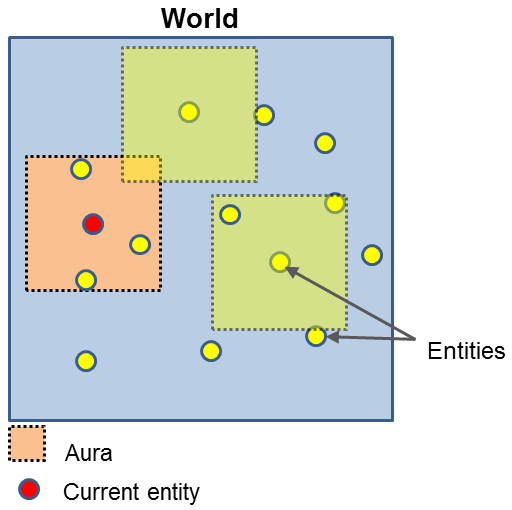
\includegraphics[width=.8\linewidth]{acm-vrst13-img/basic_area_of_interest2.png}
  \caption{Aura-based interest management.}
  %Here, each entity `sees' entities within a specified field (aura), indicated by a dotted square \cite{Prendinger+others.2014}.}
  \label{fig:basic_area}
\end{minipage}%
\begin{minipage}{.5\textwidth}
  \centering
  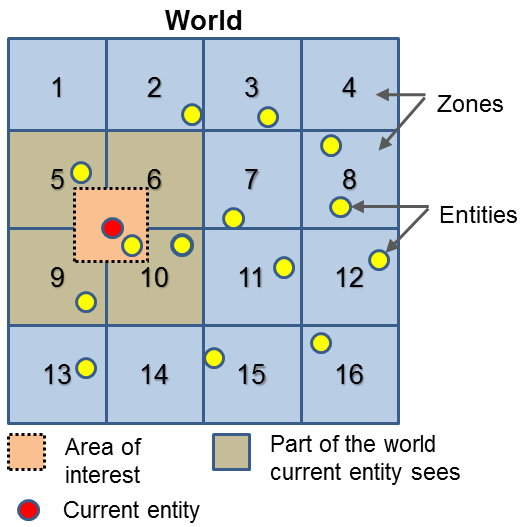
\includegraphics[width=.8\linewidth]{acm-vrst13-img/DiVE_area_of_interest2.png}
  \caption{Zone-based interest management.}
  %Here, each entity `sees' entities of all zones that its Area of Interest (indicted by dotted square) intersect \cite{Prendinger+others.2014}.}
  \label{fig:DiVE_area}
\end{minipage}
%\caption{A figure with two subfigures}
%\label{fig:test}
\end{figure}


In Fig.~\ref{fig:DiVE_area}, the current entity's AOI intersects with Zones 5, 6, 9 and 10. Therefore, it receives updates from all entities located in these zones. We can say this crosshatched group of regions is a \textit{dynamic area of interest\/} of the current entity as it changes when entity is entering/leaving (subscribing/unsubscribing) zones. The strong aspect of this implementation is that while an entity belongs to a unique zone, the entity's AOI allows it to see several regions.
In this way, we keep the number of checks small, while avoiding a situation where an entity is at the region border and sees other entities suddenly appear or disappear within very close range.

\begin{figure}[t]
\centering
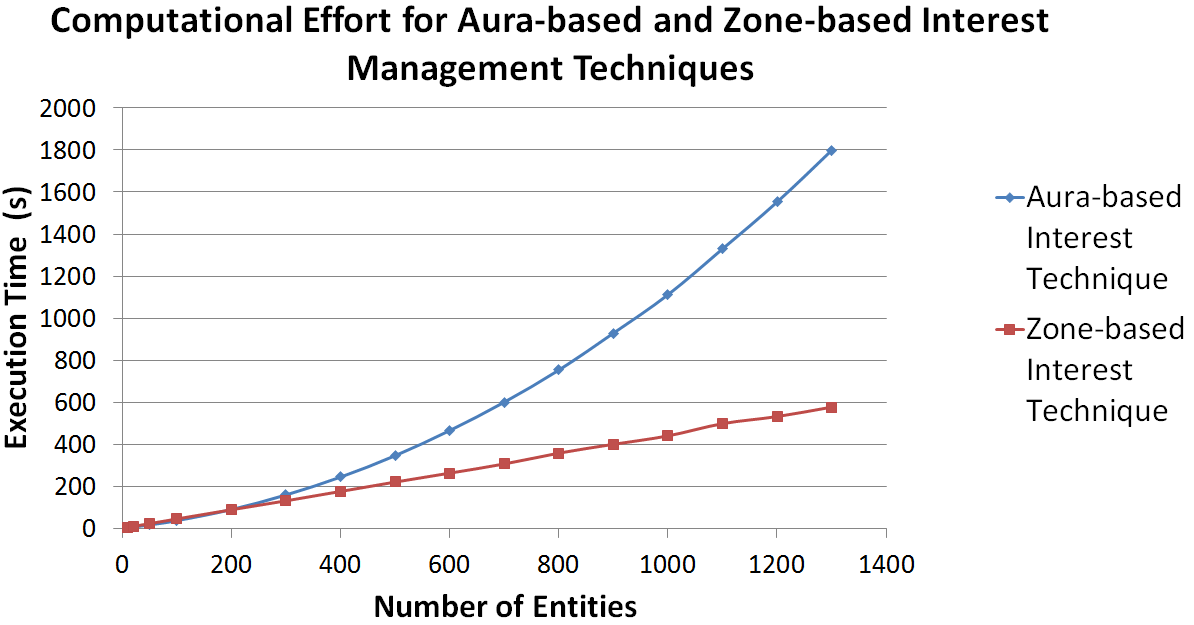
\includegraphics[width=0.8\textwidth]{acm-vrst13-img/area_comparison2.png}
\caption{Comparison of aura-based vs.~zone-based area of interest management techniques.}
\label{fig:compare_matlab}
\end{figure}



\subsection{Comparison of Aura-based and Zone-based Interest Management Techniques}

To illustrate the difference of complexity of aura-based and zone-based approaches, we implemented both methods in MATLAB.
%In the first case, an entity has an area of interest and receives updates from each entity within its range. In the second case, an entity's area of interest determines which regions the entity subscribes to and receives updates of every entities in nearby regions.
The number of zones has been fixed to sixteen.
A run consists of moving the entities pseudo-randomly for 10,000 iterations and for each frame, the interest management algorithm is activated. We used the total time of a run to compare the efficiency (as dependent variable).

{\itshape Pseudo-random} refers to a movement pattern where
\begin{itemize}
\item the entity is moving according to a randomly chosen direction and deviates slightly in a random fashion (according to a Gaussian centered on 0 deviation), and
\item a new direction is forced if the entity reaches the border of the world.
\end{itemize}
This movement pattern is close to the Brownian move with a fixed speed.
The number of entities was varied from 10 to 1300. Fig.~\ref{fig:double_threshold} indicates the quadratic complexity of the aura-based technique as opposed to the linear complexity of the zone-based approach.

\subsection{Hysteresis Mechanism}

One possible issue of this approach is the overload that is generated if an entity is oscillating between two zones. In this case, the entity enters and leaves the zone repeatedly within a short time, thereby subscribing and unsubscribing to the zone channel. The repeated forwarding of updates to the entities constitutes a redundancy in communication.

We addressed this problem by adding a hysteresis mechanism, i.e., a trigger with a moving threshold, comparable to a Schmitt trigger in electronics \cite{Schmitt.1938}. A Schmitt trigger is used to protect a mechanical actuator. If an electronic command oscillates too much, the demand on an actuator can require it to go back and forth too fast and consequently damage it. The Schmitt trigger can eliminate such undesirable effect of small oscillations.

Our specification of AOI follows a similar principle. Here, an entity has two AOI, the `inner' and the `outer' area. Figure~\ref{fig:double_threshold} shows the demand on updating the server with a standard area of interest (Case (a)) , and with the double area method (Case (b)). In Case (a), the entity enters (subscribes to) or leaves (unsubscribes from) a region each time the area of interest intersects the region. In Case (b), the entity's inner area of interest has to enter the region to belong (subscribe) to the region, whereas the entity's outer area of interest has to exit the region to notify the server that the entity left. This method prevents from flooding the server with subscribe/unsubscribe region requests.

To set the overlap size of the inner and outer area of interest, one has to consider the maximum speed of an entity. DiVE's update rate is 10 times per second (every 100ms). To avoid subscription events at every DiVE tick, the overlap should be larger than 0.1 $\times MaximumSpeed$.

\begin{figure*}[t]
\centering
%\includegraphics[width=\textwidth-30pt]{divediagram-01.pdf}
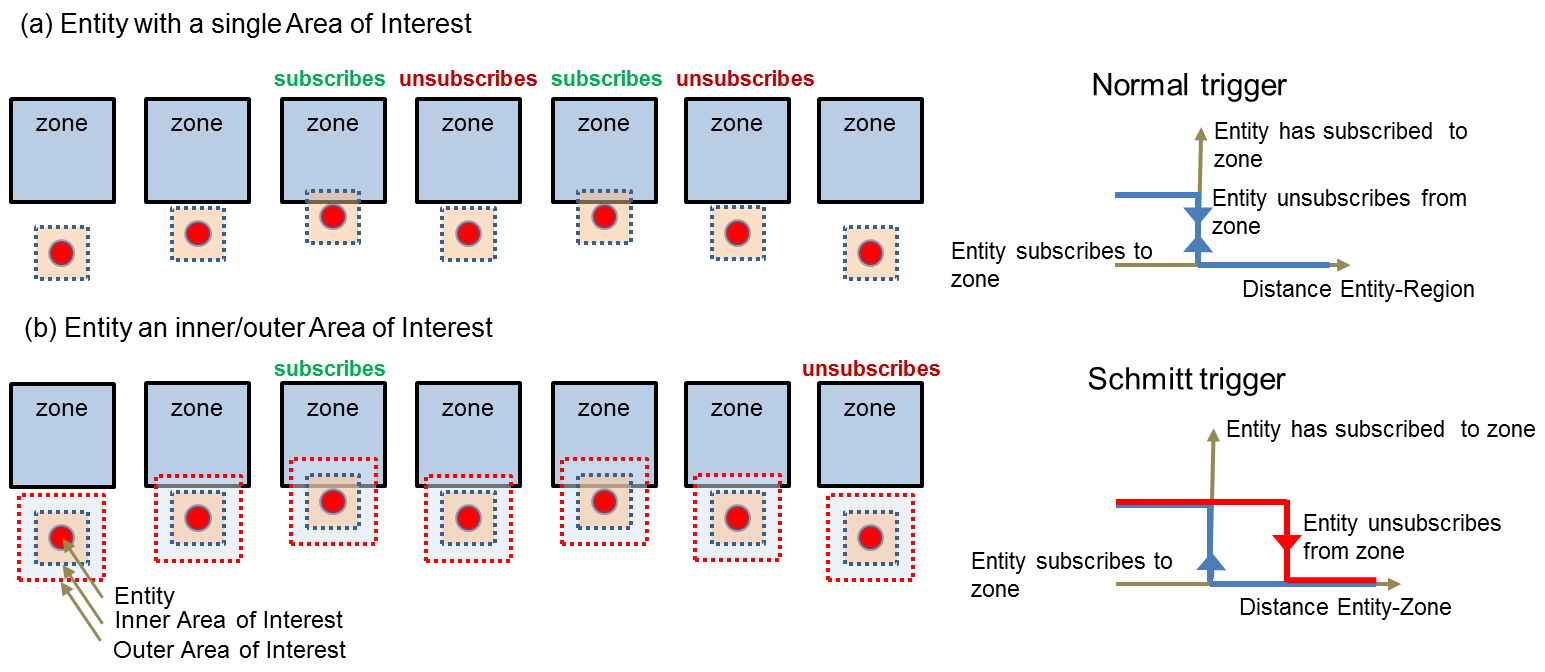
\includegraphics[width=0.95\textwidth]{acm-vrst13-img/hysteresis_description2.png}
\caption{Comparison of event triggering between a single and a double area of interest.}
\label{fig:double_threshold}
\end{figure*}


\subsection{Setting an Optimal Size for AOI}
With the zone-based approach, the number of AOI checks become independent of the number of entities on the server. However, the complexity has been moved to the zones; the more zones we have, the higher the complexity is.

Let us recall the two-fold challenge of a DVE. First, to limit the number of messages exchanged among entities; an entity should only receive relevant updates from a confined area.
Second, to limit the complexity of search method; here the zone-based model facilitates geographic sorting of entities. In this case, limiting complexity means limiting the number of zones.

So we are focusing on this part on varying the parameters of a MATLAB simulation, to study the function
\[
(t,messages,enter\_leave) = f(AOI\_ZONE,Move\_pattern)
\]
where the output elements are:
\begin{itemize}
\item $t$: the execution time of the simulation ($n$ iterations of $m$ entities, moving and receiving updates from each other every iterations).
\item $messages$: the number of exchanged messages per frame.
\item $enter\_leave$: average number of times an entity has entered/left a region
\end{itemize}

We continue with explaining the parameters.

\vspace{1.5ex}
\noindent $AOI\_ZONE$: We decided to proceed as follows. In a given multiuser application, we consider what neighborhood (surrounding) an entity may have interest in, e.g.~100m$^2$. So we chose choose 100$^2$ 100 as the AOI size.
Afterwards, the problem consists in choosing what zone size suits this AOI size.

To provide a generic way to choose the zone size, we decided to use the ratio ``AOI size / zone size''. So first we defined the AOI size, and then we varied the size of the zones, and consequently the number of zones, to find an optimum.

\vspace{1.5ex}
\noindent $Movement\_pattern$: Importantly, we want to consider different types of movement patterns and investigate how such patterns affect computation time of interest matching. First, we use two {\itshape mathematical\/} movement patterns:
\begin{itemize}
\item Pseudo-random movement pattern as explained in Section \ref{sec:AOItechnique}
\item `Checkpoint' (or `point of interest') movement pattern, where all entities share a same checkpoint list and (i) choose randomly one of these points, (ii) go to the checkpoint, and (iii) start over again.

\end{itemize}
Additionally, we consider an agent-based `social' movement pattern. In such scenario, each entity is regarded as a individual agent with various capabilities. In the preliminary implementation, the crowd of agents is divided into groups. Each group consists of a leader and members. All agents in the same group can exchange messages with each other. We implemented a message sharing agent framework based on the AgentSpeak model \cite{Rao1996}. Within the agent framework, portals provide a message management service between agents. An agent is connected to a portal which enables the agents to share messages within the same portal (see Fig.~\ref{fig:agentframe}). Initially, the agents move randomly. Once the leader starts to follow a checkpoint, it sends message to the other members in the same group to follow the checkpoint. Once the agents receive a message from a leader, the agents move towards the leaders. When the agents have arrived in the area around leader, the agents move randomly again until they receive a new message from the leader.

\begin{figure}[htb]
\centering
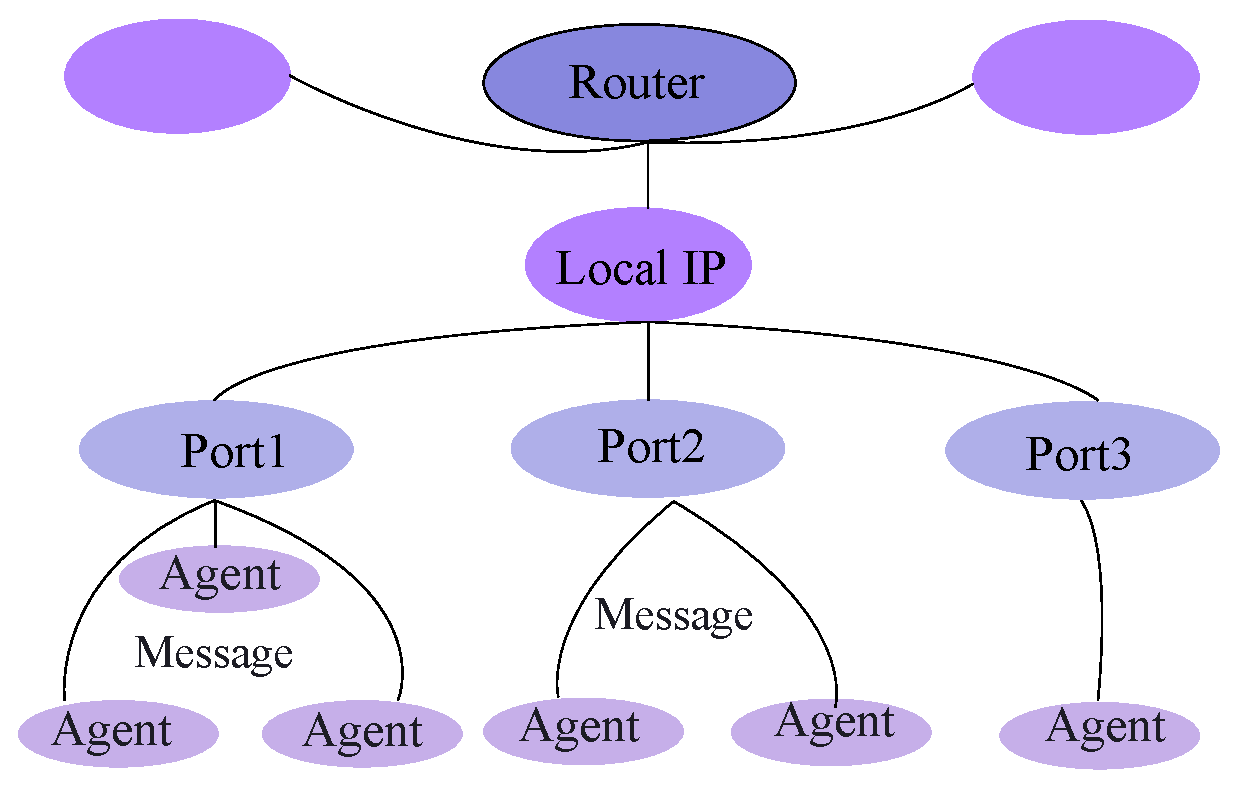
\includegraphics[width=0.7\textwidth]{acm-vrst13-img/agent-drawing.eps}
\caption{Agent framework: virtual portals (Port1, Port2, Port3) manage messaging between agents connected to same portal. Portals on different machine can share information through routers which makes the system scalable and flexible.}
\label{fig:agentframe}
\end{figure}


The experiments with the mathematical movement patterns and `social' movement pattern show some interesting findings.
Figure~\ref{fig:matlab_processing} shows the execution time of simulations (in seconds) for several ratios of AOI size and zone size. If there are few large zones, the AOI will intersect few zones, but still, the entity will see much of the world, and hence will have to update information on many entities. So, too large regions lead to significant complexity in terms of execution time. On the other hand, if we have many small zones, the number of checks on which updates have to be performed increases, and therefore the complexity is growing.
The curve is showing a low complexity between 2 and 4. Therefore, if we require to have entities with an AOI size to $x$, and choose a zone size of $x/2$.

\begin{figure}[tb!]
\centering
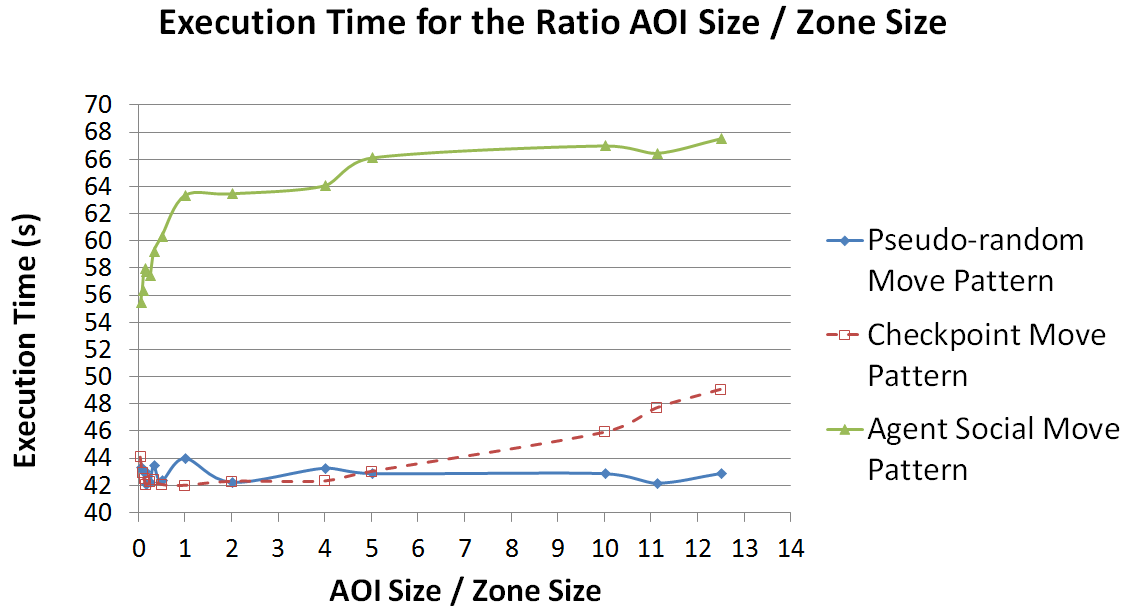
\includegraphics[width=0.95\textwidth]{acm-vrst13-img/execute-move2.png}
\caption{Processing time of the simulation, where entities move around in the virtual environment according to the number of zone (AOI is fixed).}
\label{fig:matlab_processing}
\end{figure}

We can also observe that the complexity is different depending on the move pattern. The checkpoint move pattern creates a higher load on some parts of the virtual world as the entities tend to be concentrated around the checkpoints, whereas the pseudo random move pattern tends to scatter the entities evenly on the server. Moreover, as we can see in Fig.~\ref{fig:matlab_processing},  the agent based social movement induced more complexity since each entity (agent) itself costs more computing resource as well as more message exchange. Each agent is a thread, each message portal is a thread, and each behaviour also requires a thread which increases the execution time significantly.

Figure~\ref{fig:matlab_exchanged_messages} shows the number of messages exchanged per frame and the number of ``entering/leaving zone'' events for several fractions of AOI size and zone size. We see that if there are few large zone, entities see each other frequently and more information has to be shared than with smaller zones.
On the other hand, with a higher number of smaller zones, the number of ``entering/leaving zone'' events is higher, which means that there is more communication load on the server.
Again, we notice that the a fraction around 2 is a good compromise. Also, the checkpoint movement pattern and agent movement pattern are more computationally demanding than the pseudo-random movement patterns, because entities concentrate in certain parts of the virtual world. Furthermore, we can see the event changes and message exchange of the agent social movement pattern is higher than the other two movement patterns.  Agent social movement is similar to checkpoint movement, since the agent movement pattern includes checkpoint movement as agents' initial movement. Message exchange between agents and dynamic behaviours induce additional events and message updates.

%% EDIT By Jain: I HAVE COMMENTED THIS FIGURE OUT. I THINK THIS IS WRONG. THE REIVEWERS POINTED OUT AS WELL.

%\begin{figure}[tb!]
%\centering
%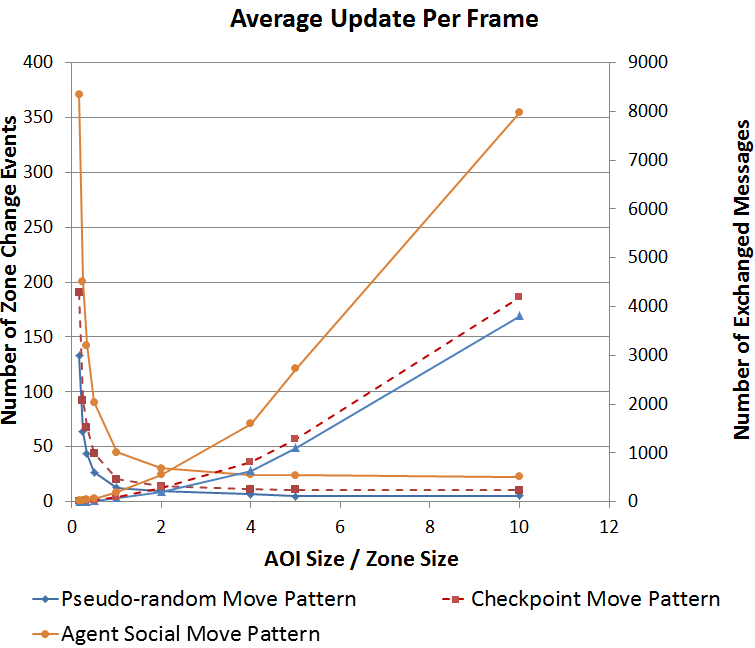
\includegraphics[width=0.8\textwidth]{acm-vrst13-img/aoi3.png}
%\caption{Number of exchanged messages and number of zone change events (entering/leaving zone) according to the size of the zone (AOI is fixed).}
%\label{fig:matlab_exchanged_messages}
%\end{figure}

\begin{figure}[tb!]
\centering
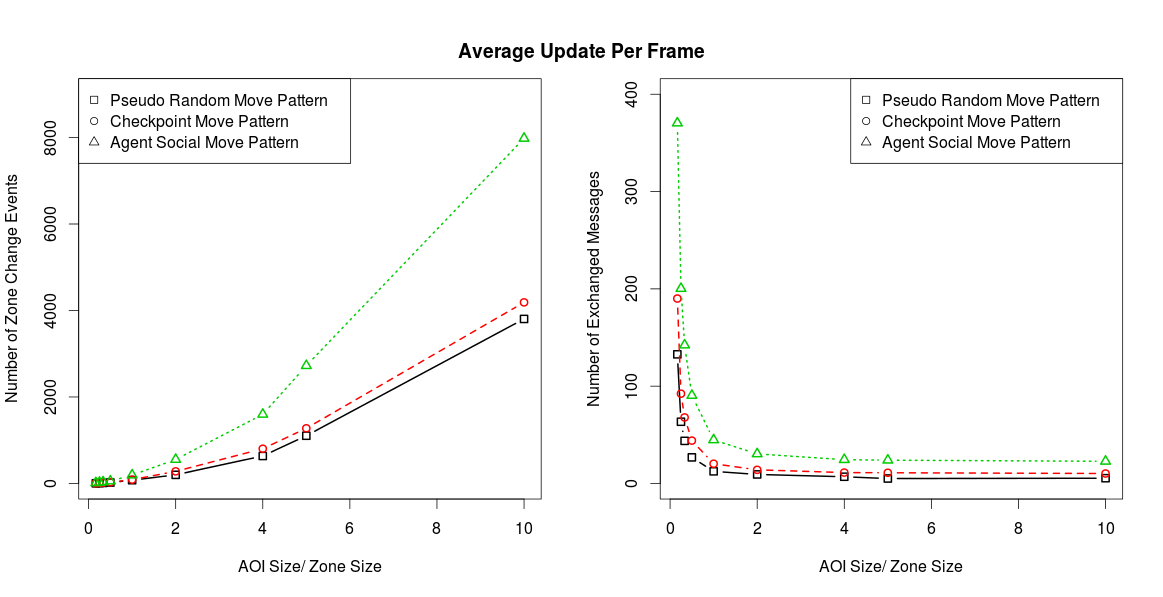
\includegraphics[width=1.0\textwidth]{acm-vrst13-img/Jain-aoi3.png}
\caption{Number of zone change events (entering/leaving zone) and the number of exchanged messages according to the size of the zone (AOI is fixed).}
\label{fig:matlab_exchanged_messages}
\end{figure}

For our experiments in Section \ref{sec:Eval}, we will use the checkpoint move pattern as a reference.

\section{DiVE Framework}\label{sec:DiVE}

DiVE aims to achieve high scalability while remaining flexible in terms of choice of operating system and compatibility with different development platforms. For efficient low-level network operations and type serialization, DiVE relies on ExitGames' Photon network middleware.\footnote{http://www.exitgames.com/} Photon consists of a server-side component and a Software Development Kit (SDK) to allow client applications communicate with the server.

The main purpose of DiVE is to efficiently share properties among defined network objects, i.e., objects that are shared across the network. In this way, DiVE maintains consistency between users in a multiuser environment. Note that an application based on DiVE must ensure that each client is using the same network objects.

DiVE has been used on several applications \cite{Madruga+others.2012,Berg+others.2012,Gajananan+others.2013,Madruga+Prendinger.2013} running with Unity3D game engine,\footnote{http://unity3d.com/}. DiVE is compatible with virtually any platform supported by the .NET and Mono common language\footnote{http://www.mono-project.com/} runtimes due to Photon's multiplatform capability. DiVE supports industry standard encryption of all transmissions.

DiVE was initially developed to conduct transport studies with multiple drivers and traffic simulation \cite{Prendinger+others.2013}.
 Preliminary systematic tests with DiVE are reported in \cite{Prendinger+others.2014}. In this paper, for the first time, we conduct an major theoretical study of the area of interest method and provide a detailed technical description of DiVE's architecture and features for application developers, including some code examples.

\subsection{DiVE Tools}

In the following we describe the tools provided by DiVE.

\begin{itemize}


\item {\itshape Generic Type Conversion\/}:
Data sharing relies on Photon's data serialization mechanism. While the number of types supported by Photon is limited, DiVE lets application developers create and register custom type converters to convert arbitrary data types used in the application. Subsequently these converters are triggered automatically by DiVE whenever an object of that type is synchronized over the network.

\item {\itshape Generic Network Event Propagation\/}:
In addition to the object-based continuous data sharing mechanism, DiVE also supports application-specific events. Conceptually, events differ from entities in that using an Entity has the goal of synchronizing between clients objects which can be updated frequently, while events are messages sent sporadically. These events encapsulate arbitrary objects courtesy of Google's Protocol Buffers\footnote{https://code.google.com/p/protobuf/} library and can thus be used to implement simple string forwarders (e.g.~for a chat function) or complex RPC components. Efficient serializers are automatically generated at compile time.

\item {\itshape Persistency\/}:
These serializers can also be used to store generic objects in a database embedded in DiVE's server component, such as user information, settings, virtual world inventories, and so on.

\item {\itshape User Authentication\/}:
User authentication can be performed with a proprietary backend or arbitrary OAuth 2.0\footnote{http://oauth.net/2/} compliant services. It also supports user management operations such as `kicking' and `banning'.

\item {\itshape Logging\/}:
A standalone .NET application functions as a generic logging client for DiVE. In order to log the data from an application, developers must create a setup file that works as a plugin to the logging. This setup determines which entities and events will be logged and how. The logging client creates an entity with maximum area of interest (monitor entity) which can see all entities in the world. From the server point of view, the logging client is just a usual client application.
\end{itemize}

\subsection{DiVE Architecture}

\begin{figure*}[t]
\centering
%\includegraphics[width=\textwidth-30pt]{divediagram-01.pdf}
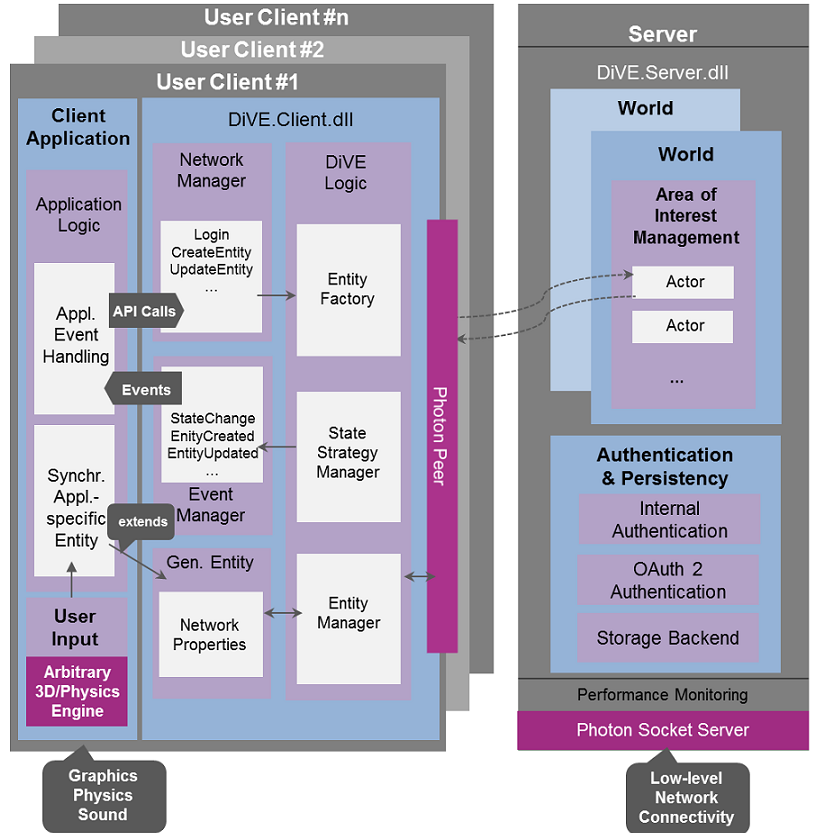
\includegraphics[width=0.9\textwidth]{acm-vrst13-img/DiVE-simple.png}
\caption{An overview of DiVE's client and server components.}
\label{fig:dive_general}
\end{figure*}

The DiVE architecture has been designed as a flexible framework that supports easy implementation of multiuser applications.
% (marconi: Removed this because it seems contradictory with the following sentence)
% DiVE requires the .NET framework 3.5.
DiVE supports both Microsoft and Mono frameworks, and hence it supports .NET and Mono based applications.

DiVE is divided into two parts: the client dll and the server dll. Fig.~\ref{fig:dive_general} shows the DiVE architecture. The server component contains 4451 C\# SLOC (Source Lines of Code), distributed among the three dlls: main application logic, persistency and area of interest management. The Client component contains 2342 C\# SLOC in a single dll. Both server and client components depend on a `common' dlls with shared types, which contains 226 C\# SLOC.

On the client side, the client dll is responsible for the synchronization of the client application with the server.
The developer decides application logic, design and graphics choices.
To interact with the client application, the client dll handles three components:
\begin{itemize}
\item \textit{NetworkManager}. Exposes DiVE's main API, with functions such as connecting and disconnecting, registering to an entity type, sharing and destroying an entity, and setting up areas of interest.

\item \textit{EventManager}. Provides a set of built-in events that the client application can listen to and that are triggered by the server. It is through the event manager that a client application knows when a new remote entity is created or destroyed, or when it is out of the sight (outside the interest area).

\item \textit{Entity}. Base class of any object that needs to be synchronized over the network. Client applications must define their own entity types, such as a CarEntity or AvatarEntity, and inherit from the \textit{Entity} class. Local entities are shared via the \textit{NetworkManager} and remote ones are received via the \textit{EventManager}.

\end{itemize}

After establishing a connection and authenticating via the \textit{NetworkManager}, a client application must `register' each of their own defined entity types with the server. Registering an entity type (e.g. the \textit{CarEntity} type), literally means telling the server that the client knows that type and is interested in sharing and/or receiving instances of that type. After registering, the client is able to share and receive entities of that type.
The basic property of the \textit{Entity} class is the \textit{position} (a 3D vector), which is used by the area of interest algorithms. All other attributes that need to be shared on the server must be declared as \textit{network properties}. After an entity instance is shared, its network properties are automatically shared via the server and updated every 0.1 seconds.

Entities should not only share their properties over the network, they should also be aware of other entities and their surrounding world. For a client application to receive updates of remote entities, it needs to setup an area of interest for its own entities. If a client application owns more than one entity, the areas of interest add up in a union fashion. To know when a remote entity was created or destroyed, a client must subscribe to events defined in the \textit{EventManager}. For example, an `entity created' event is always triggered by the server and sent to all clients who are registered to that entity type (and according to the area of interest algorithm). It is up to each client application to listen to this event and handle it.

%For that reason, DiVE is also broadcasting events across the network. Fig.~\ref{fig:event_spreading} shows how clients subscribe to events, and how they are broadcasted over the network.

Besides the built-in events from the EventManager, a client application can also define their own custom application-specific events (e.g. a chat message). Fig.~\ref{fig:event_spreading} shows how clients subscribe to events by registering their custom event type on the server. When a client triggers an event, it is broadcast over the network to all clients who registered to the same event type.

\begin{figure}[h]
\centering
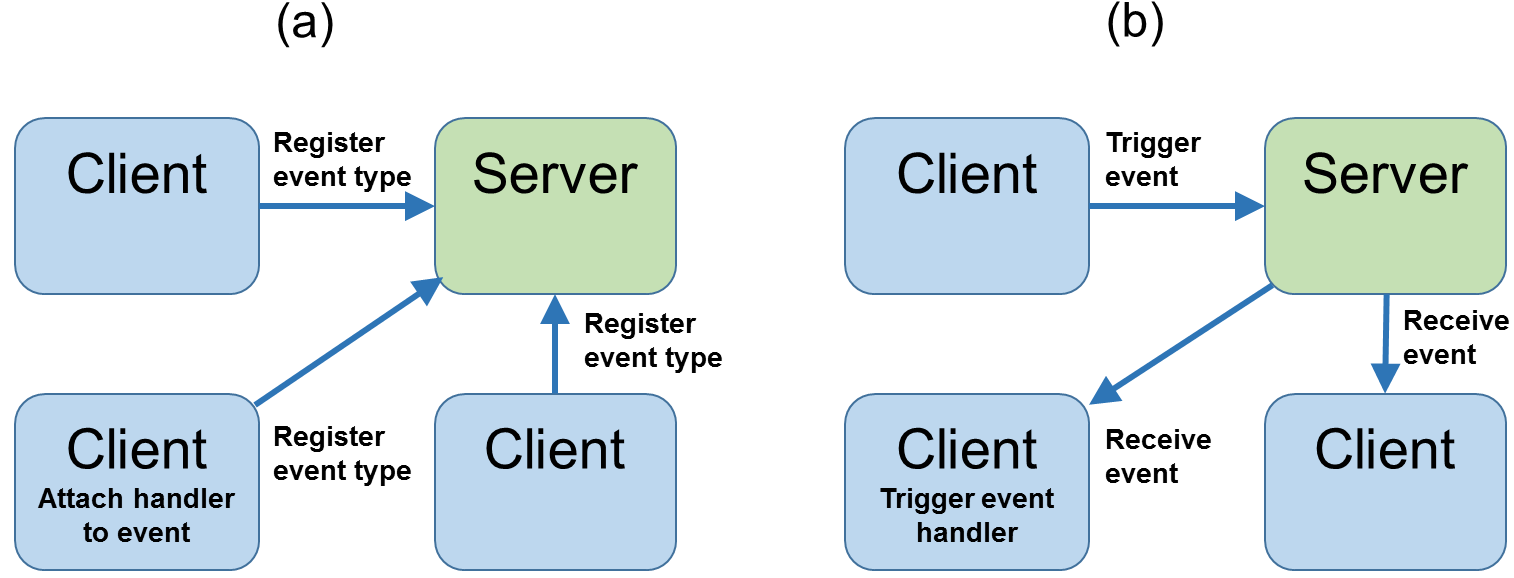
\includegraphics[width=0.6\textwidth]{acm-vrst13-img/server_request.png}
\caption{(a) Clients register custom event types and attach handlers to it; (b) a client triggers an event on the server, the server broadcasts it, and the event is captured by other clients.}
\label{fig:event_spreading}
\end{figure}

There is also the possibility for the client to create persistent objects. A persistent object is a serializable type whose state needs to be kept after the client goes offline. An example is inventory items such as virtual money. These objects will be stored on the server database.

The client application is responsible for managing the interaction with the user such as user inputs or graphic rendering, and does not have to handle network synchronization issues.
DiVE does not make a difference between a user client and a simulator-type client. That is, DiVE allows to integrate special-purpose simulators, such as traffic or pedestrian simulators, as clients. Those clients may control several entities (e.g. vehicles or pedestrians), while the user controls a single avatar. The DiVE.Client.dll is used for both kinds of clients.

On the server side, the DiVE.Server.dll has to manage the virtual world. First, it has to handle the authentication of the connection request from the DiVE client. In the case of internal authentication, the Server uses a given database of users to allow client applications to connect. When using OAuth authentication, the client application forwards the OAuth token received by the respective service(e.g. Facebook). Using this token, the server is able to retrieve information such as a user id and name, to be used within the application.

Once a client is authenticated, a respective `Actor' is created in the server side. An `Actor' is the representation of a client in the server and contains the list of entities that belong to its corresponding client. The area of interest algorithm in the server runs through actors and their entities to decide which clients will receive updates for which entities. In sequence, it sends messages to the \textit{EventManagers} in each client with property updates, creation and destruction of entities, which, in turn, triggers events to the applications.
%(marconi: Removed the log thing. This is just an error log, not relevant)
%The server dll also manages the log storage, which is useful for the detection of issues \comment{(What kind of issues?)} or even the analysis of data  from the client.
Finally, it also manages the storage of persistent objects.

%\section{Usage}

\subsection{DiVE Code Examples}

We provide code examples for two reasons. First, we want to show that it is quite easy to use DiVE to implement an application. As DiVE handles most of the network issues, the application developer only has to care about which element should be shared on the server.
Second, we want to appeal to programmers and provide complementary information to Fig.~\ref{fig:dive_general}.

The first part of the code example shown in Fig.~\ref{code1} are the type definitions. In the beginning we define the class \textit{ExampleEntity} that inherits from the DiVE class \textit{Entity}.
This means that this application deals with entities of the \textit{ExampleEntity} type and by registering it, the server will forward to this application information from other entities of the same type in the network.
\textit{ExampleEntity} has the following properties: \textit{Position} (inherited from \textit{Entity}), \textit{Rotation} and \textit{Name}.
The \textit{NetworkProperty} fields are shared with the server every 0.1 seconds. The field \textit{notSharedValue} is local to that client and will not be updated by DiVE or shared with the server as it is not a \textit{NetworkProperty}.

\begin{figure}[!tb]
\centering
\begin{lstlisting}
[Serializable]
public class ExampleEntity : Entity {
 public NetworkedProperty<float[]> Rotation { get; private set; }
 public NetworkedProperty<string> Name { get; private set; }
 private int notSharedValue;
 public ExampleEntity()
 {
  Position.Value = Vector3.one;
  Rotation = new NetworkedProperty<Vector3>(new Vector3());
  Name = new NetworkedProperty<string>(string.Empty);
 }
}
public class CustomEvent
{
  public NetworkEvent<string> MessageSent { get; private set; }

  public CustomEvent()
  {
      MessageSent = new NetworkEvent<string>();
  }
}
\end{lstlisting}
\caption{Code example showing how to easily create a network entity with DiVE. Each property declared as NetworkProperty will be shared. An example of customized network event is also given.}
\label{code1}
\end{figure}

Next, we define the class \textit{CustomEvent}, which holds a custom event defined by the application. This example event contains a string as an argument (e.g.~a broadcast chat message) that will be sent to every client that register to the \textit{CustomEvent} type. The argument of the event could be any object serializable by Google's Protocol Buffer.

The code example shown in Fig.~\ref{code2} relates to application initialization. After instantiating the \textit{EventManager} and the \textit{NetworkManager}, we connect to the server by using the \textit{NetworkManager}'s Connect() method. Since this is asynchronous, we need to subscribe to a built-in event in the \textit{EventManager} to receive the result of the connection attempt. Once we are connected, we register our \textit{ExampleEntity} and \textit{CustomEvent} types. The next step is to create and share our instance of \textit{ExampleEntity}, via the \textit{NetworkManager}'s EntityCreated() method.  To listen to our MessageSent event, we attach a local handler to it. This local function will be called by the event manager as soon as another client triggers this event.

%\comment{(I cannot easily access the content of this section, which might not be a problem. Still, I hope someone can `smoothen' it a little bit. Generally, I don't have much experience with putting such technical information in a paper. Maybe the some sentence of a concrete application or purpose might help...)}


\begin{figure}[!tb]
\centering
\begin{lstlisting}
public void Main(){
  _evtMgr = new EventManager();
  _netMgr = new NetworkManager(_evtMgr);
	
  _eventMgr.OnGameStateChange += GameStateChanged;
  _netMgr.Connect("localhost:4040"); // server IP
}

private void GameStateChanged(GameState state){
  if(state == GameState.WorldEntered){
  _netMgr.RegisterEntityType<ExampleEntity>();
  _custom = new CustomEvent();
  _netMgr.RegisterEvents<CustomEvent>(_custom);
		
  _myEntity = new ExampleEntity();
  _netMgr.EntityCreated(_myEntity);
	
  _custom.MessageSent.Event += MessageEventHandler;
  }
}
\end{lstlisting}
\caption{Code example showing how to instanciate the network classes. With the 2 code examples given, we created a network entity, sharing its name and rotation on the server.}
\label{code2}
\end{figure}

\section{Evaluation}\label{sec:Eval}

\subsection{Informal Testing of DiVE}

DiVE has already been successfully deployed in a variety of applications that use DiVE to synchronize multiple users. While those tests have been performed with human users (as clients), there was no intention or opportunity for systematic testing.

\begin{itemize}
\item Forty-one students from Hiroo Gakuen Junior and Senior High School participated in a driving behavior study on eco-safe driving practice \cite{Madruga+others.2012}.

\item Four user drivers and one hundred traffic simulator controlled cars were used to study traffic congestion caused by the `rubbernecking' effect \cite{Gajananan+others.2013}.

\item Up to forty human travelers participated simultaneously in studies on driving and travel behavior under emergency evacuation conditions \cite{Berg+others.2012}.

\item Three human drivers and twenty-seven computer-controlled `opponent' cars were involved in a multiuser eco-driving training study employing distributed constraint optimization to control the opponent cars \cite{Madruga+Prendinger.2013}.
\end{itemize}


\subsection{Systematic Testing of DiVE}

%\subsubsection{Background}

Several metrics can be used to assess the performance of a networking framework like DiVE. Previous work on the architecture of virtual worlds and on scalability used metrics like CPU usage, frames per second, bandwidth, latency and throughput \cite{Lake+others.2010,Horn+others.2010,Liu+others.2010}. Varying the number of clients and checking the value of these metrics allows us to determine how well the system handles an increase of load. Importantly, such tests can tell us at what point the user experience gets affected. Since we are dealing with interactive virtual worlds inhabited by users, it is important to identify the number of clients where the system falls below a frame rate of 30, the minimum frame rate for smooth interaction \cite{Kumar+others.2008}.

\cite{Lake+others.2010} proposed the Distributed Scene Graph (DSG) architecture, which allows scaling of actuators (processes that change the data in the scene like physics systems and clients) independently of the data (the scene itself). The main idea behind this architecture is that scalability requires that different types of processes need to be handled differently. To demonstrate the validity of their approach, the authors created a test environment with (1) a scene server holding the data of the scene, (2) five client managers, and (3) five machines with multiple clients. The client managers are processes whose main responsibility is to manage clients, which is one possible solution for scaling communication intensive processes.

The authors compared the results by running two versions, without and with the client managers. In the version using the client managers, the frame rate begins to drop with 400 clients. They showed that because there is more time spent in communication, there is also less time to handle the physics simulation. With client managers they were able to connect 750 clients before the frame rate dropped below 40 FPS. This result indicates (1) that the architecture enables the application of independent scalability techniques, evidenced by the ability to scale the clients without changing the physics simulation and (2) that scaling one part of the system has a positive impact on the remaining parts. This is expected because if we need less time to compute one part of the system (like communication), we have more time available to compute the remaining parts (like physics simulation) even if we do not scale them.

DiVE is not aimed at scaling different classes of processes because in our case, each client is responsible for rendering, physics and application logic. Our solution is targeted at scaling only the communication between processes. For that reason, we will focus on measuring how DiVE affects the rate of communication between clients and server, while keeping in mind the consequences this might have in remaining computer resources.

Using a naive approach, every entity in a virtual environment is updated about every other entity. We will refer to this approach as the `global model'. This means that whenever an entity generates information it sends a message to the remaining $n-1$ entities ($O(n(n-1))$ complexity). By using DiVE's `area of interest' notification system, we are able to reduce the complexity and consequently the amount of communication in the network. We will refer to this technique as the `local model'.

%\subsubsection{Experimental Setup}

We tested the impact of different sizes of AOI (with fixed zone size) and number of clients on the following metrics (see also \cite{Lake+others.2010}):
\begin{itemize}
\item Bandwidth as an indicator of the amount of communication;
\item Frames per second (FPS) as an indicator of the smoothness of user experience;
\item CPU and RAM usage as an indicator of the impact of our algorithm in the server machine's resources.
\end{itemize}

%Testing a DVE using only numerical metrics might be insufficient. Multiuser applications such as simulators or games have to provide a feeling of smoothness that is not sufficiently captured in the parameters described above. To ensure that our application is not lagging we decided to implement a simple 2D graphical interface that allows to observe the smoothness of the application. %Figure~\ref{fig:testEnvironment} shows a screenshot of the test environment.

We want to assess DiVE's ability to broadcast information efficiently. Therefore, for the sake of controllability, we set up our experiment in a local area network (LAN). If a lag is noticed, it can be attributed to DiVE and not to a network latency.

In summary, our testing software consists in (1) simulating clients (checkpoint movement) and (2) rendering the client's position on a 2D map, and (3) rendering the positions of the other clients and their AOI. To increase the realism of the client, the program simulates some computation (looping 1000 times) for each client.

In our tests we used a world with a 2400m$\times$2400m area with a fixed zone size of 60m$\times$60m; so there are $40\times40=1600$ regions. Then we placed the entities evenly according to their number, and moved them according to the checkpoint movement pattern, as described in Section~\ref{sec:DiVE}. The checkpoint movement pattern makes entities move inside the virtual world. As entities will typically gather around the checkpoints, we provide a sufficient number of checkpoints (50) to avoid a too high concentration of entities in some parts of the virtual world.

% Removed Figure with the 2d interface
%\begin{figure}[htb]
%\centering
%\includegraphics[width=0.49\textwidth]{acm-vrst13-img/ %screenshot2.png}
%\caption{Our test application running. Here, AOI size %is 4 times the region size.}
%\label{fig:testEnvironment}
%\end{figure}

Each client has exactly one entity. %Figure~\ref{fig:testEnvironment} shows an example of a test scenario.
As we have seen previously, the checkpoint movement pattern is slightly more heavy on the server than a pseudo-random movement pattern. In this experiment, we opted for this movement pattern because it is closer to the movement pattern in multiuser virtual worlds.
With an increasing number of clients or with a larger AOI, more entities intersect each other's AOI, which leads to an increased traffic on the network.

An ideal test scenario would use one networked machine for each client. Because this is impractical for a research lab, we devised a different approach. We use 10 different machines, each one able to connect to up to about 50 clients. The machines were running on Windows 7, and were equipped with an Intel core I7. One 11th machine was running the DiVE server while the other ten machines where running clients in parallel. The client load was divided evenly by all machines, e.g., for a scenario with 200 clients, each of the machines would host 20 clients. Our results indicate that even though running several clients in parallel in one machine affects the outcome, it is still a good approximation of the trend we would obtain if the clients were running in different machines.

\subsection{Results of Systematic Testing for DiVE 2D}

We measured the bandwidth in three runs with different sizes of AOI and with an increasing number of clients.
\begin{itemize}
\item \emph{Local AOI\/}: we use a `local' AOI, 1m$\times$1m.\footnote{Note that the client can still see the whole region where the AOI is located in.}  This size is smaller than the zone size, so the clients basically see only what is in their zone, i.e., the clients might miss some important change in the virtual environment.
\item \emph{Optimized AOI\/}: we use an `optimized' AOI according to our proposal in Section \ref{sec:DiVE}.
\item \emph{Global AOI\/}: here each client sees all other clients; there is no interest management.
\end{itemize}

\noindent {\itshape Bandwidth\/}: Figure~\ref{fig:bandwidth} shows the results for bandwidth. As expected, we obtain a weakly ascending line: the required bandwidth increases with the number of clients. Moreover, as we have seen in Section~\ref{sec:DiVE}, the growth is linear and not quadratic. Finally, the difference between using or not using interest management is obvious here. E.g., for 100 clients, interest management decreases bandwidth usage from 1200 to 60kb/s. Unfortunately, the dashed part of the `global' curve is not reliable. Indeed, above 120 clients, we started to observe strange behavior when using a global area of interest, including unexpected client disconnection, and important update loss, resulting in a very obvious latency on our 2D interface.

\begin{figure}[htb]
\centering
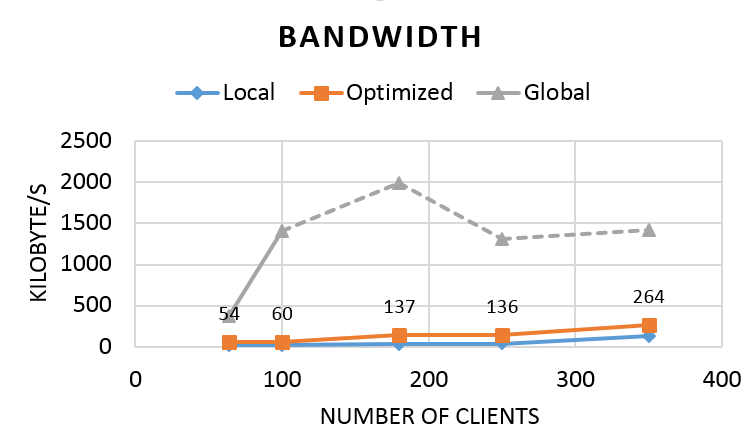
\includegraphics[width=0.6\textwidth]{acm-vrst13-img/reload_bandwidth_mod.png}
\caption{Comparison of bandwidth usage with the local and global models.}
\label{fig:bandwidth}
\end{figure}

\vspace{1.5ex}
\noindent
{\itshape Frames per second (FPS) on the clients\/}: We also wanted to test how the client interface would react to the growth of clients on the server. For that purpose, we assessed the FPS on the client side. Figure~\ref{fig:fps} illustrates that we succeed to keep the FPS high enough (above the 30 fps threshold). Again, we cannot rely on the `global' curve, insofar as above 120 clients, the connections were not reliable.

\begin{figure}[htb]
\centering
\includegraphics[width=0.6\textwidth]{acm-vrst13-img/reload_fps_mod.png}
\caption{Comparison of FPS (client) with local and global models.}
\label{fig:fps}
\end{figure}

\vspace{1.5ex}
\noindent {\itshape CPU and RAM usage on the server}: As shown by \cite{Lake+others.2010}, scaling one component of the system can also have an impact on the remaining ones. In our study we wanted to test whether our algorithm would overuse the computational resources on the server. Fig.~\ref{fig:cpu} and Fig.~\ref{fig:ram} indicate that CPU and RAM evolution with the number of clients. The memory usage is less affected by the size of the AOI, and more affected by the number of clients.

\begin{figure}[htb]
\centering
\includegraphics[width=0.6\textwidth]{acm-vrst13-img/reload_cpu_mod.png}
\caption{Comparison of CPU usage (server) with local and global models.}
\label{fig:cpu}
\end{figure}

\begin{figure}[htb]
\centering
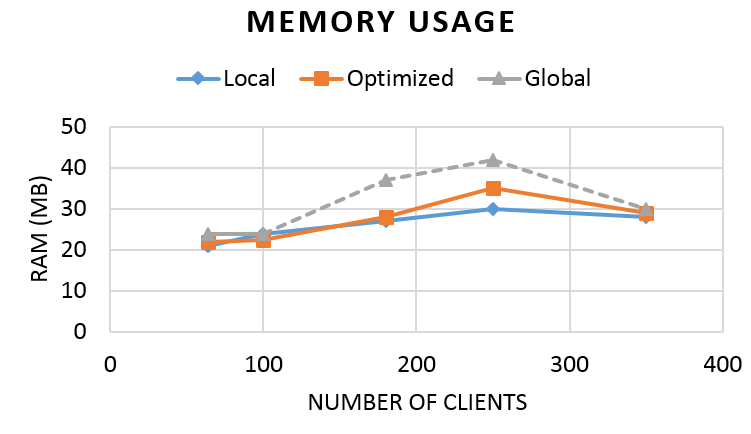
\includegraphics[width=0.6\textwidth]{acm-vrst13-img/reload_memory_mod.png}
\caption{Comparison of RAM usage (server) with local and global models.}
\label{fig:ram}
\end{figure}

It is interesting to note that the connection loss we observed above 120 client connections is not related to CPU or memory overuse, but to connection overload.
The maximum number of clients in one region is the same as the maximum number of clients with a global AOI. We started to have connection drops above 120 clients.

\subsection{Results of Systematic Testing for DiVE 3D}

\textbf{Design of the Test-Bed for DiVE 3D:} The volume of the zones does not change with the number of entities. It is set as constant to 60 m x 60 m x 60 m. The world size remains constant to 2.4 km x 2.4 km x 180 m. So, we have in total 40 x 40 x 3 = 4800 zones.  For ensuring minimal bandwidth usage, the research objective is to determine the optimal ratio of AOI volume to zone volume. For testing the causal influence of different ratios on bandwidth usage a set of ratios is chosen for our testing by varying the AOI volume. Please note that this is in contrast to our design choice of testbed for DiVE 2D in which the area of AOI is kept fixed and area of zone is variable. 

The rationale behind such design choice is because in DiVE 3d, our objective is to determine the computing needs (bandwidth consumption, CPU and RAM usage) for a single type of movement pattern which reflects the real world usage of the moving entity. For example, we intend to see how to multiple drones being used in cargo delivery task or say pick-and-place task i.e. following a check-point movement pattern can be simulated in our framework. Thus, it makes more sense to change the AOI and observe the causal influence of the number of exchanged entity-to-entity messages and entity-to-zone subscriptions on the computing needs.  On the other hand, the research objective for DiVE 2D testbed was to determine the causal influence of three different movement patterns on computing needs; thus, changing zone sizes changed the concentration of entities for each movement pattern and had causal influence on our finding.

\textbf{Experiments }
We have following two research objectives:
\begin{enumerate}
	\item \textbf{Determination of computing needs for ensuring scalability of the number of networked clients:}  This is achieved by determination of optimal ratio of volumes of AOI to Zones to ensure minimal bandwidth and CPU usage, for varying number of entities. 
	\item \textbf{Determination of suitable alignment of zones for ensuring scalability of the number of networked clients via interest management:}  Three modes of Zone alignment are used (1) Y-axis and X-Y axis and (2) No alignment, which is used in Ex 1. The performance on computing needs is compared for among the three modes. Two cases of comparisons are performed:
	\begin{itemize}
		\item \textbf{General case:} Quantitative evaluation of zone alignment on bandwidth and CPU usage for varying number of entities is tested for every ratio. The three modes are compared. 
		\item \textbf{Specific case:}  The comparison between three modes is made only for the optimal ratios (calculated as output of Ex 1).
	\end{itemize}
	
	
\end{enumerate}

\textbf{Results}

\textbf{Result of Ex1: Determination of optimal ratio:} The optimal ratio between Area of interest (AOI) and the zone is calculated. There is not distinction between inner and outer area of interest i.e. there is only one AOI. The chosen criteria for determining the optimality is minimization of the bandwidth i.e. the lower it is the more optimal the ratio.  The determination of an optimal ratio is important to find an upper bound for the ratio which has stable bandwidth. The measurement of bandwidth is required to determine the communication load on server. 

\begin{figure}[htb]
	\centering
	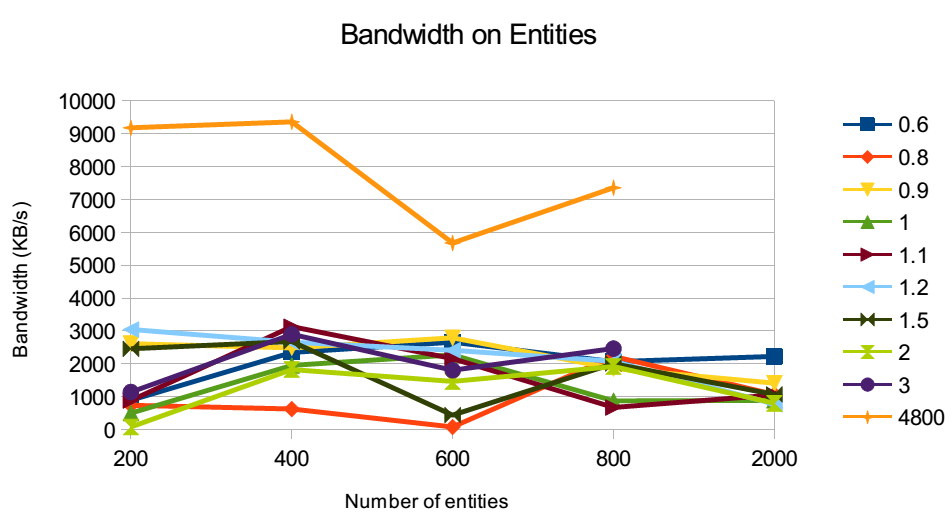
\includegraphics[width=1.0\textwidth]{acm-vrst13-img/DiVE3d-Bandwidth.png}
	\caption{Zones based interest management reduces the bandwidth consumption and ensures scaling compared to the case when there was no interest management (solid line in Orange color). For example, the client crashes when the number of entities are more than 800 and each entity sends messages to other entities (no interest management).  For a smaller number of entities i.e. 200, the optimal ratio is 2 which maintains the trade-off between exchange of messages (already limited due to small number of entities) and number of zone subscriptions (less migration from one zone to another). However, if this ratio is kept fixed and number of entities slightly increased then the number of exchanges between the entities will go up which create greater load on the server. Thus, it is preferable to have a smaller ratio (e.g. 0.8) by reducing the AOI volume since this ensures less number of zone subscriptions i.e. lesser exchange of messages. }
	\label{fig:ram}
\end{figure}

This however has a drawback of higher migration rate from one zone to another. That is why, a slight increase in ratio is found to be better for a higher number of entities.  However, it is observed that when the number of entities become very large then the choice of ratio has no substantial influence on the reduction of bandwidth usage. This can be explained as the tradeoff between the overload on server when two contrasting cases happen i.e. bigger ratio causes higher exchange of messages and smaller ratio causes higher number of zone subscriptions. 

\begin{figure}[H]
	\centering
	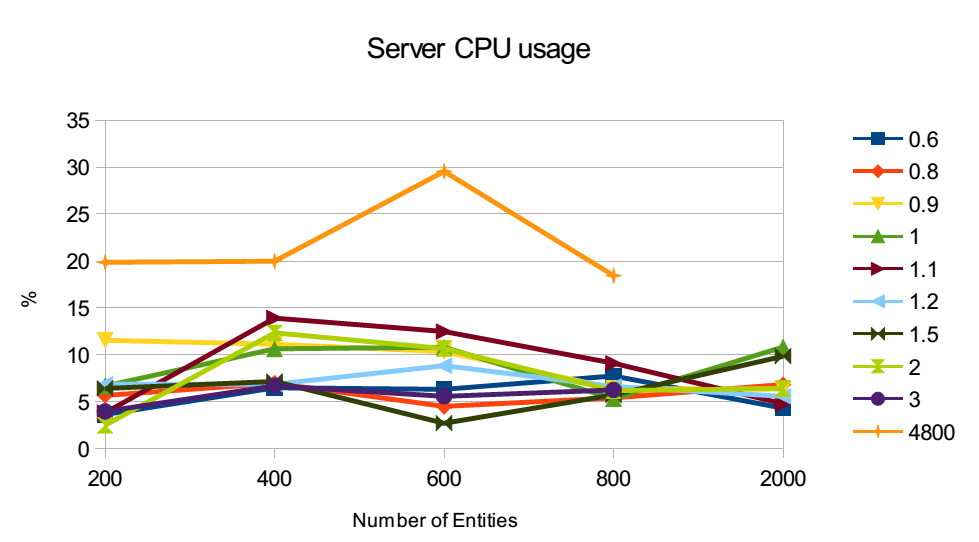
\includegraphics[width=1.0\textwidth]{acm-vrst13-img/DiVE3d-CPUUsage.png}
	\caption{Zone-based interest management reduces the CPU usage with large and small number of entities. With small number of entities i.e. 200, the CPU usage is lower and more convergent comparing to medium and large number of entities. The CPU usage converges when we have large number of entities i.e. 800. In respect to the scalability, without interest management the load of server is too heavy to perform a proper test. With interest management, we could test the entities up to 2000 with stable CPU usage. When we have the medium number of Entities i.e. 600, Rati0 1.5 costs less CPU comparing to other ratio with more obvious difference. Ratio 1.1 costs the most CPU usage when the entities are in medium number, but performs better on small and large number of entities.}
	\label{fig:ram}
\end{figure}


\textbf{Result of Ex2: Determination of suitable alignment of zones for ensuring scalability of the number of networked clients via interest management:} This experiments contains three settings, No shift, Shifted in Y axis, and Shifted in X and Y axis. The shifted width is 30 m, half of length of the region. Even order rows are shifted. In Shifted in Y axis, we would have one additional zone on shifted rows. As a result we have 4860 zones in total. In shifted in X and Y axis, we have 4901 zones. The more shift being performed, the more marginal regions would be generated. This is the natural short coming of alignment shifting.


\begin{figure}[H]
	\centering
	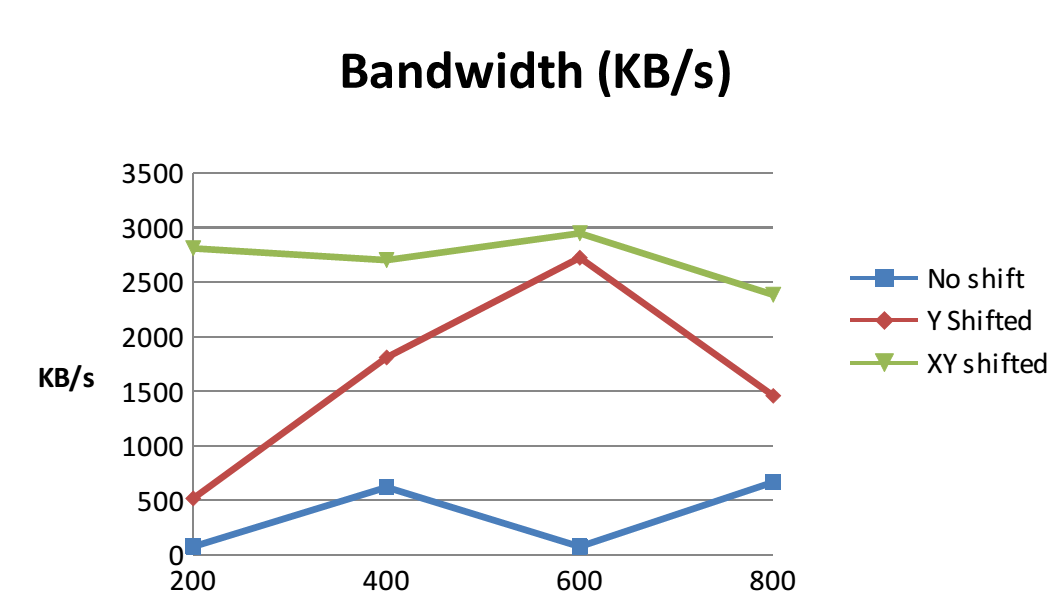
\includegraphics[width=1.0\textwidth]{acm-vrst13-img/DiVE3d-BandwidthMovementPatterns.png}
	\caption{With the optimal ratio we got using the experiment 1, we have four settings with the format (entities, ratio), (200, 2.0), (400, 0.8), (600, 0.8) and (800, 1.1). No shifted cost less bandwidth in all four settings, Shifted in Y axis performs the second best, and Shifted in both X and Y axis have most usage on bandwidth. This comes from the movement pattern that the entities have to move horizontally up and down. In such route, the Shifted contains less zones comparing to No shift. Less region lead to more entities in the same region. Thus a huge amount of bandwidth is generated.}
	\label{fig:ram}
\end{figure}

\begin{figure}[H]
	\centering
	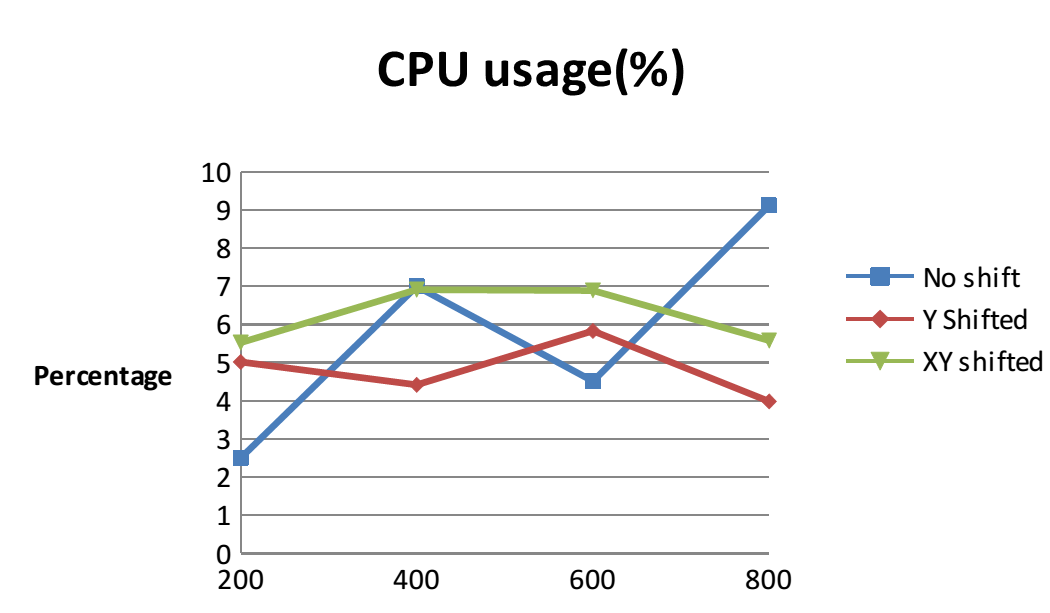
\includegraphics[width=1.0\textwidth]{acm-vrst13-img/DiVE3d-CPUMovementPatterns.png}
	\caption{With the optimal ratio we got using the experiment 1, we have four settings with the format (entities, ratio), (200, 2.0), (400, 0.8), (600, 0.8) and (800, 1.1). Shifted in Y generally use less CPU resources comparing to Shifted in X and Y. This effect could be explained by more zones are produced by shifting and thus caused more migration between zones.}
	\label{fig:ram}
\end{figure}


\begin{figure}[H]
	\centering
	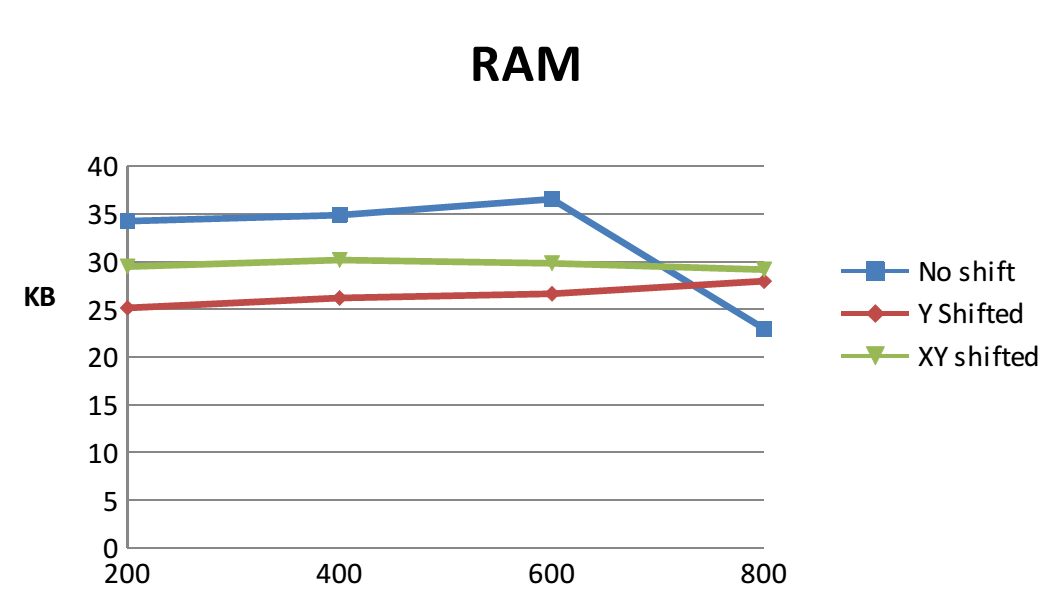
\includegraphics[width=1.0\textwidth]{acm-vrst13-img/DiVE3d-RAMMovementPatterns.png}
	\caption{With the optimal ratio we got using the experiment 1, we have four settings with the format (entities, ratio), (200, 2.0), (400, 0.8), (600, 0.8) and (800, 1.1). No shift costs more RAM than others with small amount of entities. However, when the entities goes up, it cost least RAM comparing to others. Shifted in Y costs less RAM comparing to Shifted in X and Y, but the difference shrinks when number of entities goes up.}
	\label{fig:ram}
\end{figure}



\section{Conclusions}\label{sec:Conclusions}

In the paper, we described DiVE, a simple and scalable networking framework for distributed virtual environments. DiVE is a practical framework that has already been used to implement networked multiuser applications in eco-driving \cite{Madruga+others.2012,Madruga+Prendinger.2013}, traffic accidents \cite{Gajananan+others.2013}, and evacuation \cite{Berg+others.2012}.

The focus of the paper is scalability of clients on a single-server basis. For that purpose, a zone-based Area Of Interest (AOI) technique was used and tested. First, we could demonstrate the gain from using a zone-based approach where the weight cost increases linearly with the number of entities, rather than quadratically.

Importantly, we determined an optimized (relative) value for zone size and AOI size. This value was determined empirically by simulation runs with different types of movement pattern. Besides two mathematical movement patterns (pseudo-random, checkpoint), we also use an agent-based social movement pattern. The simulations revealed 2 as the fraction of AOI size and zone size with the least number of communication across all three movement patterns.

Furthermore, the empirical evaluation of DiVE showed most promising results for the bandwidth metric. At the level of 100 users, our method outperforms a system without interest management by 20 times. The results also indicate that using interest management reduces the server CPU usage about 50\%.

Currently in DiVE, the size of the zones is fixed. To further improve scalability, we could change the number and size of zones on the server according to the number of connected clients. One solution could be to develop an algorithm spotting automatically where the crowed areas are, and partition the world accordingly.
%Our system could also be combined with \cite{Lui+Chan.2002}, so that the region shopping is distributed among several servers.

\begin{acks}
We would like to thank Martin Lindner for implementing several components of DiVE.
This work was partly supported by the `Global Lab' NII Grand Challenge grant, a Kiban Kenkyu B grant from the Japan Society of the Promotion of Science (JSPS), and by FCT (INESC-ID multiannual funding) through the PIDDAC Program PEst- OE/EEI/LA0021/2011.
\end{acks}

%\bibliographystyle{acmsiggraph}
%\section*{References}

\bibliographystyle{ACM-Reference-Format-Journals}

\bibliography{tomacs}

\end{document} 